129. \begin{figure}[ht!]
\center{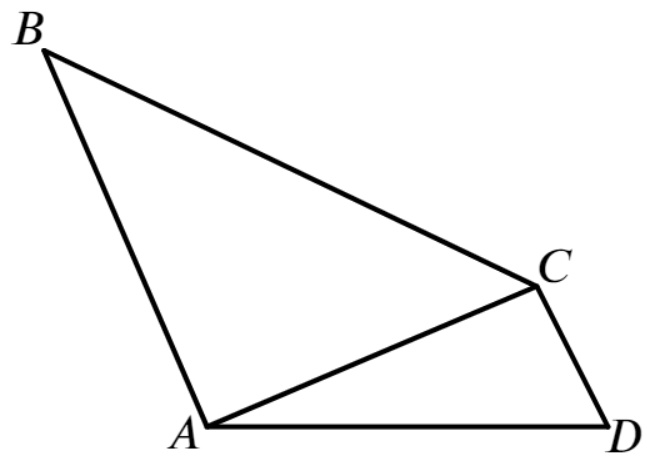
\includegraphics[scale=0.35]{g9-128.png}}
\end{figure}\\
По теореме косинусов для треугольника $ABC$ имеем $AC^2=4+9-2\cdot2\cdot3\cdot\left(-\cfrac{2}{3}
ight)=21.$ По теореме косинусов для треугольника $ACD$ получим $AC^2=49+36-2\cdot7\cdot6\cdot \cos(\angle D)=21,$ откуда $\cos(\angle D)=\cfrac{16}{21}.$\\
